%%% Choose between 16:9 and 4:3 format by commenting out/uncommenting one of the following lines:
 \documentclass[aspectratio=169]{beamer} % 16:9
%\documentclass{beamer} % 4:3

%=========================================================================================================================

\usepackage{beamerthemesplit}
\usepackage{appendixnumberbeamer}
\usepackage[ngerman]{babel}
\usepackage[utf8]{inputenc}

\usepackage{tikz}
\usepackage{url}
\usepackage{tabularx}

\useinnertheme{aig}
\useoutertheme{aig}
\usecolortheme{aig}
\usefonttheme{aig}


%=========================================================================================================================
\title{Mehrschichtige und dezentrale
Entscheidungsprozesse in Agentensystemen}
\author[H. Stadler, M. Betz]{Gruppe 3: H. Stadler, M. Betz, P. Heger und B. Wladasch}
\institute{
Fachpraktikum Künstliche Intelligenz: Multiagentenprogrammierung \\
Artificial Intelligence Group,\\
University of Hagen, Germany}
\date{30. September 2022}
%=========================================================================================================================
\logo{
\includegraphics[width=3cm]{figures/logoaig.png}}
%=========================================================================================================================

\begin{document}

%=========================================================================================================================

\begin{frame}
  \titlepage
\end{frame}
\nologo

\section*{Motivation}
\begin{frame}{Motivation}
\begin{block}{Entwicklung und Bewertung unterschiedlicher Entscheidungsprozesse von Agentensystemen im Kontext des \textit{Multi-Agent Programming Contest} 2022}
\begin{itemize}
	\item 2 Varianten basierend auf der BDI-Architektur mit unterschiedlich stark dezentralisierten Entscheidungsprozessen
	\begin{itemize}
		\item Agent V1
		\item Agent V2
	\end{itemize}
	\item Leistungsfähigkeit beider Varianten zu bewerten
	\item Verschiedene Lösungsansätze zu erhalten, die zwischen den Systemen ausgetauscht werden können
\end{itemize}
\end{block}
\end{frame}

\section{Technische Umsetzung}
\begin{frame}{Technische Umsetzung}
\begin{itemize}
\setlength\itemsep{5mm}
	\item Programmiersprache Java Version 17
	\begin{itemize}
		\item Wunsch nach umfangreichen Werkzeugen und Bibliotheken zur Verifikation und Problemfindung
	\end{itemize}
	\item Beide Agentensysteme basieren auf \textit{javaagents} Gerüst der MASSim \\ \textit{(Multi-Agent Systems Simulation Platform)}
	\item Architekturkonzepte mittels UML-Diagrammen entwickelt
	\item Projektmanagement über Github-Arbeitsablauf
	\begin{itemize}
		\item Arbeitsaufteilung über Aufgaben- und Fehlermanagement
		\item \textit{Feature-Branches} mit Quellcodeüberprüfung durch weiteres Gruppenmitglied 
	\end{itemize}
\end{itemize}
\end{frame}

\section{Agentensystem V1}
\begin{frame}{Agentensystem V1}
\frametitle{Agentensystem V1}
\begin{block}{Ziele}
\begin{itemize}
	\item Mehrschichtiger Entscheidungsprozess der das BDI-Konzept erweitert
	\item Aufbau einer umfangreichen Wissensbasis
	\item Integration der Wegfindung in den Entscheidungsprozess
	\item Strategien zur Verifikation und Problemfindung des dynamischen Systems entwickeln
\end{itemize}
\end{block}
\end{frame}
\begin{frame}{Agentensystem V1}
\frametitle{Agentensystem V1 - Architektur}
	\begin{figure}
		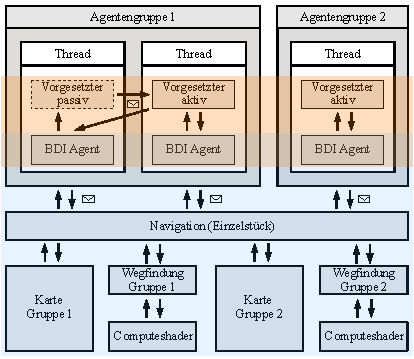
\includegraphics[scale=1]{./figures/Architekturdiagramm.pdf}
		\caption{Architektur Agentensystem V1}
		\label{debugger}
	\end{figure}
\end{frame}

\section{Agentensystem V2}
\begin{frame}{Agentensystem V2}
	\frametitle{Agentensystem V2}
	\begin{block}{Struktur}
	\end{block}
	\textbf{ }
	\begin{itemize}
		\setlength\itemsep{5mm}
		\item Der AgentV2 arbeitet mit der Step-Methode		
		\item Desires mit und ohne Task-Bezug
	\end{itemize}
	\begin{table}
	\small
	\begin{tabular}{lll}
		\textbf{ohne Task} & \textbf{mit Task} & \textbf{Mehr\-Block\-Task}\\
		LocalExploreDesire & GoAbandonedBlockDesire & MasterMultiBlocksDesire\\
		GoAdoptRoleDesire & GoDispenserDesire & HelperMultiBlocksDesire\\
		ExploreMapSizeDesire & GoGoalZoneDesire & Helper2MultiBlocksDesire\\
		& SubmitDesire & ConnectMultiBlocksDesire\\
	\end{tabular}
	\end{table}
\end{frame}

\begin{frame}{Agentensystem V2}
	\frametitle{Agentensystem V2}
	\begin{block}{Wie finden die Agenten ihre Desires?}
	\end{block}
	\textbf{ }
	\begin{itemize}
		\setlength\itemsep{5mm}
		\item In jedem Step werden alle Desires auf Ausführbarkeit geprüft		
		\item Alle ausführbaren Desires bekommen dynamisch eine Priorität vergeben
		\item Das Desire mit der höchsten Priorität wird zur Intention
		\item Aus der Intention wird die nächste Aktion des Agenten abgeleitet
	\end{itemize}
\end{frame}

\begin{frame}{Agentensystem V2}
	\frametitle{Agentensystem V2}
	\begin{block}{Wie arbeiten die Agenten zusammen?}
	\end{block}
	\textbf{ }
	\begin{itemize}
		\setlength\itemsep{5mm}
		\item Bildung von Supervisor-Gruppen bei jedem Treffen fremder Agenten		
		\item Bildung von dynamischen Adhoc-Kooperationen innerhalb der Supervisor-Gruppen zur Bearbeitung einer Task
		\item Keine zentrale Koordination der Agenten
		\item Steuern der Art und Anzahl der Adhoc-Kooperationen über Setup-Variablen
		\item Nutzung der Adhoc-Kooperationen auch zur Ermittlung der Mapgröße
	\end{itemize}
\end{frame}

\section{Turniere}

\section{Rekapitulation und Ausblick}

\begin{frame}{Blocks}
    \begin{block}{Block}
        This is a regular block.
        \begin{itemize}
            \item This is an item in a block.
        \end{itemize}
    \end{block}
    
    \begin{alertblock}{Block}
        This is an alert block.
        \begin{itemize}
            \item This is an item in an alert block.
        \end{itemize}
    \end{alertblock}
    
    \begin{exampleblock}{Block}
        This is an example block.
        \begin{itemize}
            \item This is an item in an example block.
        \end{itemize}
    \end{exampleblock}
\end{frame}


\begin{frame}{Highlighting Text}
    We can \highlight{highlight} text. There are also a \darkhighlight{darker} option, and a \yellowhighlight{yellow} option.\\
    The same options are also available in math mode: $\mathhighlight{a} + \darkmathhighlight{b} = \yellowmathhighlight{c}$
\end{frame}


\appendix

\section{Appendix}

\begin{frame}{Appendix}
    This is an appendix.
    \begin{itemize}
        \item Page numbers start from the beginning.
    \end{itemize}
\end{frame}

\end{document}
